\documentclass[12pt,a4paper]{article}

% ─── Packages ─────────────────────────────────────────────────────────────────
\usepackage[utf8]{inputenc}
\usepackage[T1]{fontenc}
\usepackage{lmodern}
\usepackage[margin=2.5cm]{geometry}
\usepackage{amsmath,amssymb,amsthm}
\usepackage{microtype}
\usepackage{setspace}
\usepackage{parskip}
\usepackage[hidelinks,
            pdftitle={Literature Review: Lévy Scaling of Futures Price Increments},
            pdfauthor={}]{hyperref}
\usepackage{tikz}
\usetikzlibrary{shapes.geometric, arrows.meta, positioning, calc}
\usepackage[style=authoryear,
            backend=biber,
            maxbibnames=99,
            maxcitenames=2,
            uniquelist=false,
            giveninits=true,
            doi=true,
            url=false]{biblatex}
\addbibresource{references.bib}

\onehalfspacing

\begin{document}

% ── Pipeline figure ───────────────────────────────────────────────────────────
\begin{figure}[htbp]
\centering
% Scale to text width so the figure always fits regardless of margin settings
\resizebox{\textwidth}{!}{%
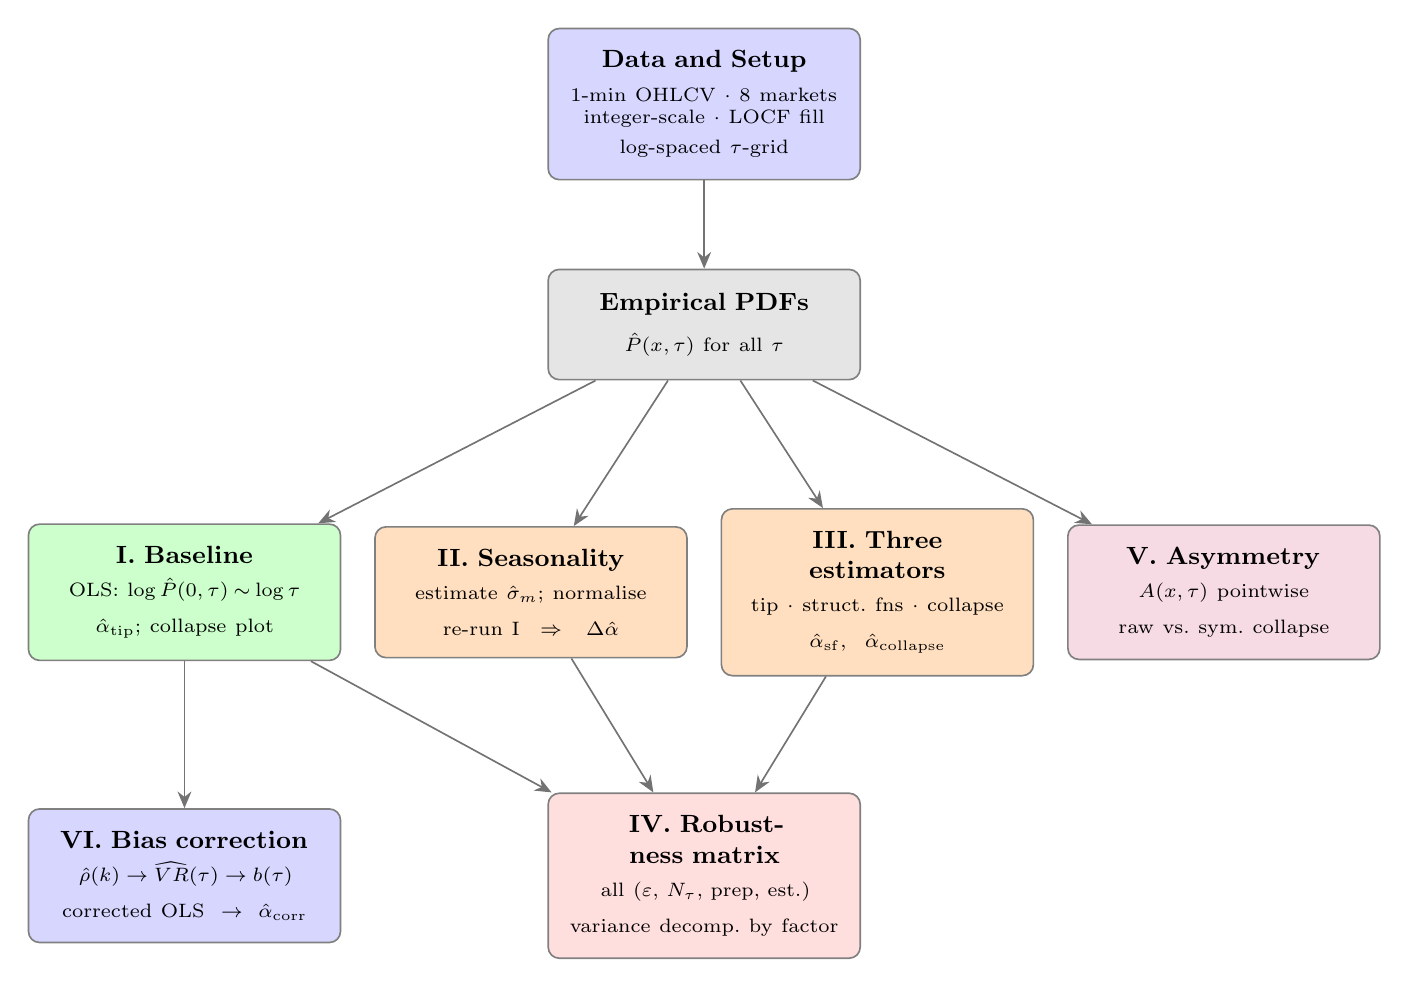
\begin{tikzpicture}[
  % Default box style; colour supplied per node as box=<colour>
  box/.style={
    rectangle, rounded corners=4pt,
    draw=black!50, semithick,
    fill=#1,
    text width=3.4cm, align=center,
    inner sep=8pt, minimum height=1.4cm,
    font=\small
  },
  arr/.style={-{Stealth[length=6pt,width=5pt]}, black!55, semithick},
]

%% ── Row 0: data input ──────────────────────────────────────────────────────
\node[box=blue!16] (data) at (0,0) {
  \textbf{Data and Setup}\\[4pt]
  \scriptsize
  1-min OHLCV $\cdot$ 8 markets\\
  integer-scale $\cdot$ LOCF fill\\
  log-spaced $\tau$-grid
};

%% ── Row 1: shared intermediate ────────────────────────────────────────────
\node[box=gray!20] (pdfs) at (0,-2.8) {
  \textbf{Empirical PDFs}\\[4pt]
  \scriptsize $\hat{P}(x,\tau)$ for all $\tau$
};

%% ── Row 2: four parallel analyses ─────────────────────────────────────────
%  Centres spaced 4.4 cm apart; boxes are ~3.9 cm wide → ~0.5 cm gap each side
\node[box=green!20] (s1) at (-6.6,-6.2) {
  \textbf{I.\ Baseline}\\[4pt]
  \scriptsize
  OLS: $\log\hat{P}(0,\tau)\!\sim\!\log\tau$\\[2pt]
  $\hat{\alpha}_{\mathrm{tip}}$; collapse plot
};

\node[box=orange!25] (s2) at (-2.2,-6.2) {
  \textbf{II.\ Seasonality}\\[4pt]
  \scriptsize
  estimate $\hat{\sigma}_m$; normalise\\[2pt]
  re-run I $\;\Rightarrow\; \Delta\hat{\alpha}$
};

\node[box=orange!25] (s3) at (2.2,-6.2) {
  \textbf{III.\ Three estimators}\\[4pt]
  \scriptsize
  tip $\cdot$ struct.\ fns $\cdot$ collapse\\[2pt]
  $\hat{\alpha}_{\mathrm{sf}},\;\hat{\alpha}_{\mathrm{collapse}}$
};

\node[box=purple!14] (s5) at (6.6,-6.2) {
  \textbf{V.\ Asymmetry}\\[4pt]
  \scriptsize
  $A(x,\tau)$ pointwise\\[2pt]
  raw vs.\ sym.\ collapse
};

%% ── Row 3: outputs ────────────────────────────────────────────────────────
%  VI sits under I; IV sits under II+III (centre of their span = −2.2+2.2)/2 = 0)
\node[box=blue!16] (s6) at (-6.6,-9.8) {
  \textbf{VI.\ Bias correction}\\[4pt]
  \scriptsize
  $\hat{\rho}(k)\!\to\!\widehat{VR}(\tau)\!\to\!b(\tau)$\\[2pt]
  corrected OLS $\;\to\;\hat{\alpha}_{\mathrm{corr}}$
};

\node[box=red!13] (s4) at (0,-9.8) {
  \textbf{IV.\ Robustness matrix}\\[4pt]
  \scriptsize
  all $(\varepsilon,\,N_\tau,\,\mathrm{prep},\,\mathrm{est.})$\\[2pt]
  variance decomp.\ by factor
};

%% ── Arrows ────────────────────────────────────────────────────────────────
\draw[arr] (data) -- (pdfs);
\draw[arr] (pdfs) -- (s1);
\draw[arr] (pdfs) -- (s2);
\draw[arr] (pdfs) -- (s3);
\draw[arr] (pdfs) -- (s5);
\draw[arr] (s1)   -- (s4);
\draw[arr] (s2)   -- (s4);
\draw[arr] (s3)   -- (s4);
\draw[arr] (s1)   -- (s6);

\end{tikzpicture}%
}% end resizebox
\caption{Analytical pipeline. All six sections operate on the same empirical
PDF table constructed in the data-and-setup phase. Sections~II-V are parallel
tests of the Section~I baseline under different perturbations (preprocessing,
estimator choice, model-assumption validity). Section~IV aggregates the
sensitivity results from Sections~I-III into a single variance decomposition.
Section~VI corrects the Section~I tip estimator for the upward bias induced by
short-term autocorrelation.}
\label{fig:pipeline}
\end{figure}
% ─────────────────────────────────────────────────────────────────────────────
\end{document}